\subsubsection{問題設定}
計測対象として,拍動周期$T$の非圧縮性のニュートン流体による流れを考える.
ここでは3次元を考え,MRI領域$\Omega_{\text{m}} \subseteq \mathbb{R}^3$における
ボクセルの大きさを$\Delta x_{\mathrm{m}} \times \Delta y_{\mathrm{m}} \times \Delta z_{\mathrm{m}}$
とし,1周期中の計測数を$N_m$回とする計測間隔$\Delta t_{\text{m}}$).
また,ボクセル$i$,時刻$t_{j} \in(0, T]$におけるMRI速度を$\mathbf{v}^{ij}_{\mathrm{m}}$と定義する.
これに対し,数値計算を適用する計算領域を$\Omega \subseteq \mathbb{R}^3$とし,
座標 $\mathbf{x} \in \Omega$ ,時刻 $t \in(0, T]$ での
数値速度を$\mathbf{v}(\mathbf{x}, t) \in \mathbf{H}_{0,\Gamma_{\mathrm{w}}}^1(\Omega)$と定義する.
データ同化の制御変数には,$t=0$における数値計算の初期速度場$\mathbf{v}_0$と,
入口境界$\Gamma_{\mathrm{I}}$における境界速度$\mathbf{V}(t)$を用いる.

目的関数を
\begin{equation}
    \label{eq:cost_function_unsteady}
    \mathcal{J}(\mathbf{v}, \mathbf{v}^{0}, \mathbf{V}) 
    = \mathcal{D}(\mathbf{v}) + \mathcal{R}(\mathbf{v}^{0}, \mathbf{V})
\end{equation}
と定義する.右辺第1項は,計測速度と数値速度の時空間情報に対する誤差の和
\begin{equation}
    \label{eq:error_function_unsteady}
    \mathcal{D}(\mathbf{v}) = 
    \frac{\alpha}{2} \sum_{j=1}^{N_\text{m}} \sum_{i=1}^{M_\text{m}} 
    \left\|\mathcal{T}^{\text{ave}}_{ij} \mathbf{v}(\mathbf{x},t) 
    - \mathbf{v}_\text{m}^{ij}\right\|^2 \Delta x_m \Delta y_m \Delta z_m \Delta t_m
\end{equation}
であり,$\alpha$は誤差関数のハイパーパラメータである.$\mathcal{T}^{\text{ave}}_{ij}$は
Tögerら\cite{Toger2020}を参考にし,時空間方向の平滑化を考慮した計測オペレータ
\begin{equation}
    \label{eq:operator_average_unsteady}
    \mathcal{T}^{\text{ave}}_{ij}  : \mathbf{v}(\mathbf{x},t) 
    \mapsto \left(\int_{t} \ w^{j}_{t} \ dt\right)^{-1}
    \left(\int_{\Omega} \ w^{i}_{\Omega} \ d \Omega\right)^{-1} 
    \int_{T} \int_{\Omega} \mathbf{v}(\mathbf{x},t) \ w^{i}_{\Omega} w^{j}_{t} \ d \Omega dt
\end{equation}
とする.ここで,$w^{i}_{t}$と$w^{i}_{\Omega}$は時間方向と空間方向の重み関数であり,
Fig. 3.\ref{fig:smoothing}にそれぞれの関数を示す.
また,これらの式は
\begin{align}
    & \begin{aligned}
        w^{i}_{\Omega}
        & = \text{sinc}\left(\frac{x-x_i}{\Delta x_{m}}\right) \text{sinc}\left(\frac{y-y_i}{\Delta y_{m}}\right) \text{sinc}\left(\frac{z-z_i}{\Delta z_{m}}\right) \\
        & \times \mathcal{X}\left(x;x_{i},4\Delta x_{m}, \sigma_{\mathrm{xyz}}\right)\mathcal{X}\left(y;y_{i},4\Delta y_{m}, \sigma_{\mathrm{xyz}}\right)\mathcal{X}\left(z;z_{i},4\Delta z_{m}, \sigma_{\mathrm{xyz}}\right) 
        \label{eq:operator_weight_space_unsteady}
    \end{aligned} \\[5pt]
    & \begin{aligned}
        w^{j}_{t}
        = \mathcal{X}\left(t;t_{j}, \Delta t_{m}, \sigma_{t}\right)
        \label{eq:operator_weight_time_unsteady}
    \end{aligned}
\end{align}
と表される.ここで,$\mathcal{X}$は平滑化関数として
\begin{equation}
    \mathcal{X}\left(a; a_{0}, w, \sigma\right) 
    = \frac{1}{1+e^{-\left(a - \left(a_{0} - w/2 \right)\right) / \sigma}}-\frac{1}{1+e^{-\left(a - \left(a_{0} + w/2 \right)\right) / \sigma}}
\end{equation}
と定義される.$a$適当な変数,$a_{0}$は対称軸の値,$w$と$\sigma$はパラメータである.
目的関数のおける右辺第2項は正則化項を表し,各制御変数に対するノルムとして
\begin{equation}
    \label{eq:regularization_unsteady}
    \begin{aligned}
    \mathcal{R}(\mathbf{v}^0, \mathbf{V}) 
    &= \frac{\beta}{2} \int_{T}  \int_{\Gamma_\mathrm{I}} \Bigl[\left\|\partial_t{\mathbf{V}}\right\|^2+\left\|\partial_s \mathbf{V}\right\|^2 \Bigr] \, d\Gamma dt
    + \frac{\gamma}{2} \int_{\Omega}  \left\|\partial_s \mathbf{v}^{0} \right\|^2 \, \mathrm{d}\Omega
    \end{aligned}
\end{equation}
と定義する.

\begin{figure}[H]
    \begin{center}
      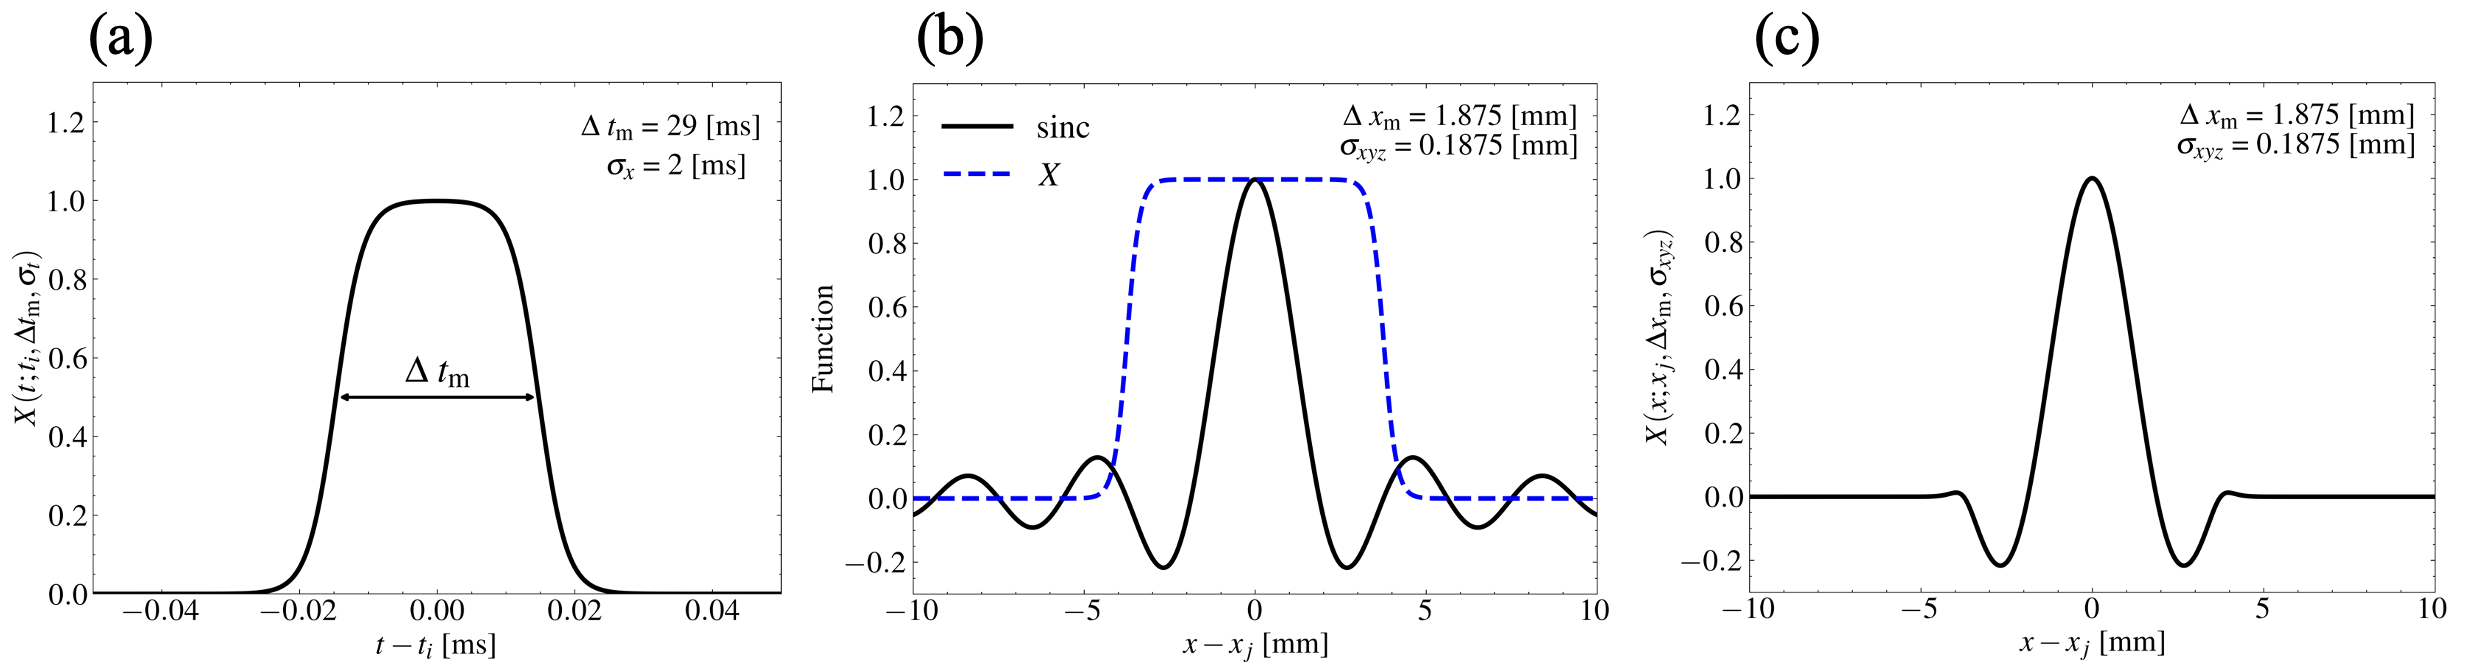
\includegraphics[width=1.0\textwidth]{figures/smoothing.png}
    \end{center}
    \caption{Smoothing functions used in the observation operator 
    $\mathcal{T}^{\mathrm{ave}}$ \cite{Toger2020}. 
    (a) Thetemporal smoothing function consisted of a box-like function with smoothed edges. 
    The width was set to the temporal resolution of the 4D flow MRI data. 
    (b) Spatial smoothing function - sinc function (continuous line) 
    and smoothed truncation (dashed line). 
    (c) Spatial smoothing function - final truncated form.}
    \label{fig:smoothing}
\end{figure}

\subsubsection{支配方程式}
流体の支配方程式を,ナビエ・ストークス方程式と連続の式を用いて
\begin{equation}
    \label{eq:govering_eq_unsteady}
    \begin{aligned}
    \rho \partial_t \mathbf{v} + \rho \mathbf{v} \cdot \nabla \mathbf{v} + \nabla p - \mu \nabla^2 \mathbf{v} + \frac{1}{\rho} \mathbf{K}(\phi) \mathbf{v} =0 & \hspace{1em} \text { in } \Omega \times (0, T]  \\
    \nabla \cdot \mathbf{v} = \mathrm{0} & \hspace{1em} \text { in } \Omega  \times (0, T] 
    \end{aligned}
\end{equation}
と記述する.

\subsubsection{変分法}
式(\ref{eq:govering_eq_unsteady})をSUPG/PSPG法により,
\begin{equation}
    \label{eq:weak_form_unsteady}
    \begin{aligned}
        \mathcal{F}\bigl(\mathbf{v}, p, \mathbf{V}, \mathbf{w}, q, \bm{\lambda}, \bm{\eta}\bigr)
        & =\;
        \int_{\Omega} \Bigl[
            \rho\, \mathbf{w} \cdot \partial_t \mathbf{v}
            \;+\; \rho\, \mathbf{w} \cdot \bigl(\mathbf{v} \cdot \nabla \mathbf{v}\bigr)
            \;-\; p\, (\nabla \cdot \mathbf{w})
            \;+\; \mu\, \nabla \mathbf{w} : \nabla \mathbf{v}
            \;+\; \mathbf{w} \cdot \mathbf{K}\, \mathbf{v}
        \Bigr] \,\mathrm{d}\Omega \\
        &
        + \int_{\Omega} 
            q\, (\nabla \cdot \mathbf{v})
        \,\mathrm{d}\Omega
        + \smash{\sum_{e=1}^{M}}
        \int_{\Omega_{e}} \Bigl[
            \rho\, \tau_{e}\,
              \bigl(\mathbf{v} \cdot \nabla \mathbf{w}\bigr)
              \cdot
              \bigl(\mathbf{v} \cdot \nabla \mathbf{v}\bigr)
            \;+\;
              \rho\, \tau_{e}\,
              \bigl(\mathbf{v} \cdot \nabla \mathbf{w}\bigr)
              \cdot
              \partial_t \mathbf{v} \\
            & \;+\;
            \tau_{e}\,
              \bigl(\mathbf{v} \cdot \nabla \mathbf{w}\bigr)
              \cdot
              \nabla p 
            +\;
            \tau_{e}\,
            \nabla q \cdot 
            \partial_t \mathbf{v}
            +\;
            \tau_{e}\,
            \nabla q \cdot 
            \bigl(\mathbf{v} \cdot \nabla \mathbf{v}\bigr)
            \;-\;
            \frac{\tau_{e}}{\rho}\,
            \nabla q \cdot
            \nabla p
        \Bigr]\,\mathrm{d}\Omega \\
        &
        - \int_{\Gamma_{\mathrm{I}}} \Bigl[
            \bm{\lambda} \cdot \bigl(\mathbf{v} - \mathbf{V}\bigr)
            \;+\;
            \bm{\eta} \cdot \bigl(\mathbf{w} - \mathbf{0}\bigr)
        \Bigr]\,\mathrm{d}\Gamma
    \end{aligned} 
\end{equation} 
と記述し,最適化における拘束条件とする.出口境界にはtraction-freeを仮定した.
煩雑を避けるため,以降の定式ではSUPG/PSPG項は省略する.
目的関数・拘束条件を合わせたLagrange関数を
\begin{equation}
    \label{eq:lagrange_unsteady}
    \mathcal{L}\left(\mathbf{v}, p, \mathbf{v}_{0}, \mathbf{V}, \mathbf{w}, q, \bm{\lambda}, \bm{\eta}\right)
    =\mathcal{J}\left(\mathbf{v}, \mathbf{v}_{0}, \mathbf{V}\right) - \int_{T}\mathcal{F}\left(\mathbf{v}, p, \mathbf{V}, \mathbf{w}, q, \bm{\lambda}, \bm{\eta}\right)dt
\end{equation}
とし,制約なし最小化問題を
\begin{equation}
    \label{eq:minimization}
    \min_{\mathbf{v}^{0}, \mathbf{V}} \mathcal{L}
\end{equation}
と定義する.

式(\ref{eq:lagrange_unsteady})の時間方向の離散化を考える.
はじめに,誤差関数におけるボクセルi,計測点jでの
誤差を$\mathbf{v}^{ij}_{\mathrm{e}}$
と表す.誤差は各計測点の離散和であるため
\begin{equation}
    \label{eq:error_function_spline_interpolated}
    \begin{aligned}
        \frac{\alpha}{2} \sum_{j=1}^{N_\text{m}} \sum_{i=1}^{M_\text{m}} 
        \|\mathbf{v}^{ij}_{\mathrm{e}}\|^2 \Delta x_m \Delta y_m \Delta z_m \Delta t_m
        \approx \frac{\alpha}{2} 
        \int_{T} 
        \sum_{i=1}^{M_\text{m}} 
        \|\mathbf{v}^{i}_{\mathrm{e}}\|^2 
        \Delta x_m \Delta y_m \Delta z_m 
        dt
    \end{aligned}
\end{equation}
として時間方向の連続関数とする.ここで$\mathbf{v}^{i}_{\mathrm{e}}$は
ボクセルiにおける,3次スプラインによる補間関数である.
次に,式(\ref{eq:lagrange_unsteady})を
数値計算の時間刻み$\Delta t$で時間離散化すると
\begin{align}
    \label{eq:discretized_lagrange_unsteady}
    \mathcal{L} 
    \;=\; \sum_{k=1}^{N} \mathcal{T}_{k} \, \Delta t
    \;-\; \sum_{k=0}^{N-1} \mathcal{F}_{k} \, \Delta t
    \;+\; \frac{\gamma}{2} \int_{\Omega} \left\|\partial_s \mathbf{v}^{0} \right\|^2 \, \mathrm{d}\Omega
\end{align}
と表せる.$N$は数値計算の総ステップ数である.
ここで,$\mathcal{T}_{k}$は,時間ステップ$k \ (1 \leq k \leq N)$における
初期条件の正則化項を除いた目的関数であり
\begin{equation}
    \label{eq:cost_function_discretized}
    \mathcal{T}_{k}
    = \frac{\alpha}{2} 
    \sum_{i=1}^{M_\text{m}} 
    \|\mathbf{v}^{ik}_{\mathrm{e}}\|^2
    \Delta x_m \Delta y_m \Delta z_m 
    \;+\; \frac{\beta}{2}
    \int_{\Gamma_\mathrm{I}} 
    \Bigl[
        \bigl\|\frac{\mathbf{V}^{k+1}-\mathbf{V}^k}{\Delta t}\bigr\|^2
        +
        \bigl\|\partial_s \mathbf{V}^{k}\bigr\|^2
    \Bigr]
    d \Gamma
\end{equation}
と表す.また,$\mathcal{F}_{k}$は時間ステップ$k \ (0 \leq k \leq N-1)$における
拘束条件であり
\begin{equation}
    \label{eq:weak-form-k}
    \begin{aligned}
        \mathcal{F}_{k} & = \int_{\Omega} \bigg[\mathbf{w}^{k+1}
        \cdot \rho \frac{\mathbf{v}^{k+1}-\mathbf{v}^k}{\Delta t} 
        + \mathbf{w}^{k+1} \cdot \rho \left(\frac{3\mathbf{v}^{k} - \mathbf{v}^{k-1}}{2}\right) 
        \cdot \nabla \left(\frac{\mathbf{v}^{k} + \mathbf{v}^{k-1}}{2}\right) + p^{k+1} (\nabla \cdot \mathbf{w}^{k+1}) \\
        &- \mu\nabla\mathbf{w}^{k+1} : \nabla \left(\frac{\mathbf{v}^{k} + \mathbf{v}^{k-1}}{2}\right)
        + \mathbf{w}^{k+1} \cdot \frac{1}{\rho}\mathbf{K}(\phi) \left(\frac{\mathbf{v}^{k} + \mathbf{v}^{k-1}}{2}\right)+ q^{k+1}(\nabla \cdot \mathbf{v}^{k+1})\bigg] \, \mathrm{d}\Omega \\
        &- \int_{\Gamma_{\text{I}}} \lambda^{k+1} \cdot (\mathbf{v}^{k+1} - \mathbf{V}^{k+1}) \, \mathrm{d}\Gamma - \int_{\Gamma_1} \boldsymbol{\eta}^{k+1} \cdot (\mathbf{w}^{k+1} - \mathbf{0}) \, \mathrm{d}\Gamma = \mathbf{0}
    \end{aligned}
\end{equation}
と表す.ここで,時間微分項に対して1次オイラー法を用い,
移流項,粘性項,Darcy項にはCrank-Nicolson法を用いて離散化した.
また,移流速度を2次精度Adams-Bashforth法により線形化した.\par
制御変数の感度導出にあたり,随伴変数法を用いる.
主問題は,$\mathbf{w}$,$q$,$\boldsymbol{\lambda}$に関するガトー微分より,
\begin{equation}
    \everymath{\displaystyle}
    \setlength{\arraycolsep}{0.5pt}
    \renewcommand{\arraystretch}{2.5}
    \label{eq:main_problem}
    {}^{t}\!\left\langle\frac{\partial \mathcal{L}}{\partial \mathbf{w}}, \delta {\mathbf{w}}\right\rangle
    = \begin{pmatrix}
        \left\langle\frac{\partial \mathcal{L}}{\partial \mathbf{w}^{\scriptscriptstyle 1}}, \delta {\mathbf{w}}^{\scriptscriptstyle 1}\right\rangle \\
        \vdots \\
        \left\langle\frac{\partial \mathcal{L}}{\partial \mathbf{w}^{\scriptscriptstyle N}}, \delta {\mathbf{w}}^{\scriptscriptstyle N}\right\rangle 
    \end{pmatrix}
    =\mathbf{0}
    ,\quad
    {}^{t}\!\left\langle\frac{\partial \mathcal{L}}{\partial q}, \delta {q}\right\rangle
    = \begin{pmatrix}
        \left\langle\frac{\partial \mathcal{L}}{\partial q^{\scriptscriptstyle 1}}, \delta {q}^{\scriptscriptstyle 1}\right\rangle \\
        \vdots \\
        \left\langle\frac{\partial \mathcal{L}}{\partial q^{\scriptscriptstyle N}}, \delta {q}^{\scriptscriptstyle N}\right\rangle 
    \end{pmatrix}
    =\mathbf{0}
    ,\quad
    {}^{t}\!\left\langle\frac{\partial \mathcal{L}}{\partial \boldsymbol{\lambda}}, \delta \boldsymbol{\lambda}\right\rangle
    = \begin{pmatrix}
        \left\langle\frac{\partial \mathcal{L}}{\partial \boldsymbol{\lambda}^{\scriptscriptstyle 1}}, \delta \boldsymbol{\lambda}^{\scriptscriptstyle 1}\right\rangle \\
        \vdots \\
        \left\langle\frac{\partial \mathcal{L}}{\partial \boldsymbol{\lambda}^{\scriptscriptstyle N}}, \delta \boldsymbol{\lambda}^{\scriptscriptstyle N}\right\rangle 
    \end{pmatrix}
    =\mathbf{0}
\end{equation}
と表され,時間ステップ$k \ (1 \leq k \leq N)$において
\begin{align}
    &\begin{aligned}
        \label{eq:foward_w}
        \left\langle\frac{\partial \mathcal{L}}{\partial \mathbf{w}^k}, \delta {\mathbf{w}}^k\right\rangle
        &= \int_{\Omega} \Bigl[\delta {\mathbf{w}}^{k} \cdot \rho\frac{\mathbf{v}^{k}-\mathbf{v}^{k-1}}{\Delta t}
        +\delta {\mathbf{w}}^{k} \cdot \rho \left(\frac{3\mathbf{v}^{k} - \mathbf{v}^{k-1}}{2}\right) \cdot \nabla \left(\frac{\mathbf{v}^{k} + \mathbf{v}^{k-1}}{2}\right) \\
        &+ p^{k} (\nabla \cdot \delta {\mathbf{w}}^{k})
        - \mu \nabla \delta {\mathbf{w}}^{k} : \left(\frac{\mathbf{v}^{k} + \mathbf{v}^{k-1}}{2}\right)
        + \delta {\mathbf{w}}^{k} \cdot \frac{1}{\rho}\mathbf{K}(\phi) \left(\frac{\mathbf{v}^{k} + \mathbf{v}^{k-1}}{2}\right) \Bigr] \, \mathrm{d}\Omega \\
        &- \int_{\Gamma_1} \boldsymbol{\eta}^{k} \cdot \delta {\mathbf{w}}^{k} \, \mathrm{d}\Gamma = 0
    \end{aligned} \\
    \label{eq:foward_q} 
    & \left\langle\frac{\partial \mathcal{L}}{\partial q^k}, \delta {q}^k\right\rangle
    =\int_{\Omega} \delta {q}^k(\nabla \cdot \mathbf{v}^{k+1}) \, \mathrm{d}\Omega
    = 0 \\
    \label{eq:foward_lambda} 
    &\left\langle\frac{\partial \mathcal{L}}{\partial \boldsymbol{\lambda}^k}, \delta \boldsymbol{\lambda}^k\right\rangle
    = \int_{\Gamma_1} \delta \boldsymbol{\lambda}^k \cdot (\mathbf{v}^{k} - \mathbf{V}^{k}) \, \mathrm{d}\Gamma
    = 0
\end{align}
とそれぞれ記述できる.

次に,随伴問題は,$\mathbf{v}$,$p$,$\boldsymbol{\eta}$に関するガトー微分より
\begin{equation}
    \everymath{\displaystyle}
    \setlength{\arraycolsep}{0.5pt}
    \renewcommand{\arraystretch}{2.5}
    \label{eq:adjoint_problem}
    {}^{t}\!\left\langle\frac{\partial \mathcal{L}}{\partial \mathbf{v}}, \delta \mathbf{v}\right\rangle
    = \begin{pmatrix}
        \left\langle\frac{\partial \mathcal{L}}{\partial \mathbf{v}^{\scriptscriptstyle 1}}, \delta \mathbf{v}^{\scriptscriptstyle 1}\right\rangle \\
        \vdots \\
        \left\langle\frac{\partial \mathcal{L}}{\partial \mathbf{v}^{\scriptscriptstyle N}}, \delta \mathbf{v}^{\scriptscriptstyle N}\right\rangle 
    \end{pmatrix}
    =\mathbf{0}
    ,\quad
    {}^{t}\!\left\langle\frac{\partial \mathcal{L}}{\partial p}, \delta p\right\rangle
    = \begin{pmatrix}
        \left\langle\frac{\partial \mathcal{L}}{\partial p^{\scriptscriptstyle 1}}, \delta p^{\scriptscriptstyle 1}\right\rangle \\
        \vdots \\
        \left\langle\frac{\partial \mathcal{L}}{\partial p^{\scriptscriptstyle N}}, \delta p^{\scriptscriptstyle N}\right\rangle 
    \end{pmatrix}
    =\mathbf{0}
    ,\quad
    {}^{t}\!\left\langle\frac{\partial \mathcal{L}}{\partial \boldsymbol{\eta}}, \delta \boldsymbol{\eta}\right\rangle
    = \begin{pmatrix}
        \left\langle\frac{\partial \mathcal{L}}{\partial \boldsymbol{\eta}^{\scriptscriptstyle 1}}, \delta \boldsymbol{\eta}^{\scriptscriptstyle 1}\right\rangle \\
        \vdots \\
        \left\langle\frac{\partial \mathcal{L}}{\partial \boldsymbol{\eta}^{\scriptscriptstyle N}}, \delta \boldsymbol{\eta}^{\scriptscriptstyle N}\right\rangle 
    \end{pmatrix}
    =\mathbf{0}
\end{equation}
と表せる.時間ステップ$k \ (1 \leq k \leq N)$では
\begin{align}
    &\begin{aligned}
        \label{eq:adjoint_v}
        \left\langle\frac{\partial \mathcal{L}}{\partial \mathbf{v}^k}, \delta \mathbf{v}^k\right\rangle
        & = \int_{\Omega} \Bigl[ \rho\frac{\mathbf{w}^{k} - \mathbf{w}^{k+1}}{\Delta t} \cdot \delta \mathbf{v}^k
        + \frac{\rho}{4} \mathbf{w}^{k} \cdot \left( 3\mathbf{v}^{k-1} - \mathbf{v}^{k-2} \right) \cdot \nabla \delta \mathbf{v}^{k}
        + \frac{3\rho}{4} \mathbf{w}^{k+1} \cdot \delta \mathbf{v}^k \cdot \nabla \mathbf{v}^{k+1} \\ 
        & + \frac{\rho}{4} \mathbf{w}^{k+1} \cdot \left( 3\mathbf{v}^k - \mathbf{v}^{k-1} \right) \cdot \nabla \delta \mathbf{v}^{k}
        - \frac{\rho}{4} \mathbf{w}^{k+2} \cdot \delta \mathbf{v}^{k} \cdot \nabla \mathbf{v}^{k+1} 
        - \frac{\rho}{4}  \mathbf{w}^{k+2} \cdot \delta \mathbf{v}^{k} \cdot \nabla \mathbf{v}^{k} \\
        & - \frac{\mu}{2} \left(\nabla \mathbf{w}^{k} + \nabla \mathbf{w}^{k+1}\right) : \nabla \delta \mathbf{v}^k
        + \frac{1}{2\rho} \left(\mathbf{w}^{k} + \mathbf{w}^{k+1}\right) \cdot \mathbf{K}(\phi) \delta \mathbf{v}^k 
        \Bigr] \, \mathrm{d}\Omega \\
        & + q^{k} (\nabla \cdot \delta \mathbf{v}^{k}) 
        + \int_{\Gamma_1} \lambda^{k} \cdot \delta \mathbf{v}^{k} \, \mathrm{d}\Gamma
        = \alpha \smash{\sum_{i=1}^{M_\text{m}}}
        \mathbf{v}^{ik}_{\mathrm{e}}
        \cdot \delta \mathbf{v}^k 
        \Delta x_m \Delta y_m \Delta z_m 
    \end{aligned} \\
    \label{eq:adjoint_p} 
    & \left\langle\frac{\partial \mathcal{L}}{\partial p^k}, \delta p^k\right\rangle
    =\int_{\Omega} \delta p^k(\nabla \cdot \mathbf{w}^{k}) \, \mathrm{d}\Omega 
    = 0 \\
    \label{eq:adjoint_eta} 
    &\left\langle\frac{\partial \mathcal{L}}{\partial \boldsymbol{\eta}^k}, \delta \boldsymbol{\eta}^k\right\rangle
    =\int_{\Gamma_1} \delta \boldsymbol{\eta}^k \cdot \mathbf{w}^k \, \mathrm{d}\Omega 
    = 0
\end{align}
とそれぞれ書き下せる(Appendix A).ここで,式(\ref{eq:adjoint_v})に関して
\begin{equation}
    \label{eq:adjoint_eq_condition}
    \begin{cases}
        \displaystyle \mathbf{v}^{k-2} = \mathbf{v}^{0} & \text{for } k=1 \\
        \displaystyle \mathbf{w}^{k+2} = \mathbf{0} & \text{for } k=N-1 \\
        \displaystyle \mathbf{w}^{k+1} = \mathbf{w}^{k+2} = \mathbf{0} & \text{for } k=N
    \end{cases}
\end{equation}
であり,$k = N$の場合のみ$\mathbf{w}^{k+1}$もしくは$\mathbf{w}^{k+2}$
の時間ステップに依存せず独立に連立方程式が解けることから,随伴方程式は時間逆発展方程式となる.
最後に,主問題,随伴問題より得た変数から,初期速度と,時間ステップ$k \ (1 \leq k \leq N)$における入口境界速度の感度
\begin{align}
    \label{eq:adjoint_v0}
    &\begin{aligned}
        \left\langle\frac{\partial \mathcal{L}}{\partial \mathbf{v}^0}, \delta \mathbf{v}^0\right\rangle
        = & \gamma \int_{\Omega}  \big( \mathbf{v}^{0} \cdot \delta \mathbf{v}^0 
        + \partial_s \mathbf{v}^{0} \cdot \delta \mathbf{v}^0 \big) \, \mathrm{d}\Omega
        + \int_{\Omega} \bigg( \rho\frac{ \mathbf{w}^{1}}{\Delta t} \cdot \delta \mathbf{v}^0
        - \frac{3\rho}{4} \mathbf{w}^{1} \cdot \delta \mathbf{v}^0 \cdot \nabla \mathbf{v}^{1}
        - \frac{\rho}{2} \mathbf{w}^{1} \cdot \mathbf{v}^0 \cdot \nabla \delta \mathbf{v}^{k} \\
        &+ \frac{\rho}{4} \mathbf{w}^{2} \cdot \delta \mathbf{v}^{0} \cdot \nabla \mathbf{v}^1
        + \frac{\rho}{4} \mathbf{w}^{2} \cdot \delta \mathbf{v}^{0} \cdot \nabla \mathbf{v}^{0}
         + \frac{\mu}{2} \nabla \mathbf{w}^{1} : \nabla \delta \mathbf{v}^0
        - \frac{1}{2\rho} \mathbf{w}^{1} \cdot \mathbf{K}(\phi) \delta \mathbf{v}^0 
        \bigg) \, \mathrm{d}\Omega 
    \end{aligned} \\
    &\left\langle\frac{\partial \mathcal{L}}{\partial \mathbf{V}^k}, \widetilde{\mathbf{V}}^k\right\rangle
    = \beta \int_{\Gamma_\mathrm{I}} \big( \mathbf{V}^k \cdot \widetilde{\mathbf{V}}^k + \partial_s \mathbf{V}^k \cdot \widetilde{\mathbf{V}}^k + \dot{\mathbf{V}}^k \cdot \widetilde{\mathbf{V}}^k + \partial_s \dot{\mathbf{V}} \cdot \widetilde{\mathbf{V}}^k \big) \, \mathrm{d}\Gamma
    - \int_{\Gamma_\mathrm{I}} \lambda \cdot \widetilde{\mathbf{V}}^k \mathrm{d} \Gamma
\end{align}
を導出し,これらを用いて,制御変数を
\begin{equation}
    \mathbf{v}^0_{n+1} = \mathbf{v}^0_n - \tau_1\left\langle\frac{\partial \mathcal{L}}{\partial \mathbf{v}^0}, \delta \mathbf{v}^0\right\rangle
\end{equation}
\begin{equation}
    \mathbf{V}^k_{n+1}=\mathbf{V}^k_n - \tau_2\left\langle\frac{\partial \mathcal{L}}{\partial \mathbf{V}^k}, \delta \mathbf{v}^k\right\rangle
\end{equation}
と最急降下法に基づき逐次更新する.$n$は最適化ステップ数を表し,$\tau_1$と$\tau_2$はArmijo条件\cite{Armijo1966}より決定したそれぞれの更新幅である.\par
空間離散化については,定常流の場合と同様に有限要素法を用いた.

